%%%%%%%%%%%%%%%%%%%%%%%%%%%%%%%%%%%%%%%%%%%%%%%%%%%%%%%%%%%%
%% This poster is based on a template I found online when %%
%% trying to figure out how to make a poster in LaTeX.    %%
%% This template can be found in this folder in the       %%
%% compressed file ``confposter.tgz''. This poster        %%
%% requires the ``a0size'' and ``textpos'' macros         %%
%% included in that file, that are of course also present %%
%% in this directory so the document will compile.        %%
%%%%%%%%%%%%%%%%%%%%%%%%%%%%%%%%%%%%%%%%%%%%%%%%%%%%%%%%%%%%
\documentclass{article}

% load packages
\usepackage{amsmath}
\usepackage{pstricks}
\usepackage[absolute]{textpos}
\usepackage{graphicx}
\usepackage{times}
\usepackage[usenames]{color}
\usepackage{a0size}
\usepackage{url}

% define colors
\newrgbcolor{darkblue}{0.1 0.1 0.5}
\definecolor{darkblue}{rgb}{0.1,0.1,0.5}
\definecolor{black}{rgb}{0.0,0.0,0.0}
\definecolor{red}{rgb}{0.9,0.0,0.1}
\definecolor{darkblue2}{rgb}{0.00,0.08,0.6}
\definecolor{darkred}{rgb}{0.6,0.00,0.08}
\definecolor{darkgreen}{rgb}{0.00,0.6,0.08}

% definitions
\let\Textsize\normalsize
\def\RHead#1{\noindent\hbox to \hsize{\hfil{\LARGE\color{darkblue}
#1}}\bigskip}
\def\LHead#1{\noindent{\LARGE\color{darkblue} #1}\bigskip}
\def\CHead#1{\begin{center}\noindent{\LARGE\color{darkblue} #1}\end{center}}
\def\Subhead#1{\noindent{\large\color{darkblue} #1}\bigskip}
\def\Title#1{\noindent{\textbf{\veryHuge\color{darkgreen} #1}}}

% suppress page numbers
\pagestyle{empty} 

% paper size
\setlength{\paperwidth}{40in}
\setlength{\paperheight}{30in}
\setlength{\textwidth}{36in}
\setlength{\textheight}{26in}
\special{papersize=\the\paperwidth,\the\paperheight}

% margins
\setlength{\headheight}{0cm}
\setlength{\headsep}{0cm}
\setlength{\topmargin}{1in}
\setlength{\topskip}{0cm}
\setlength{\oddsidemargin}{1in}
\setlength{\evensidemargin}{0in}

% font sizes
\renewcommand{\tiny}{\fontsize{12}{14}\selectfont}
\renewcommand{\scriptsize}{\fontsize{14.4}{18}\selectfont}   
\renewcommand{\footnotesize}{\fontsize{17.28}{22}\selectfont}
\renewcommand{\small}{\fontsize{20.74}{25}\selectfont}
\renewcommand{\normalsize}{\fontsize{24.88}{30}\selectfont}
\renewcommand{\large}{\fontsize{29.86}{37}\selectfont}
\renewcommand{\Large}{\fontsize{35.83}{45}\selectfont}
\renewcommand{\LARGE}{\fontsize{43}{54}\selectfont}
\renewcommand{\huge}{\fontsize{51.6}{64}\selectfont}
\renewcommand{\Huge}{\fontsize{61.92}{77}\selectfont}
\newcommand{\veryHuge}{\fontsize{74.3}{93}\selectfont}
\newcommand{\VeryHuge}{\fontsize{89.16}{112}\selectfont}
\newcommand{\VERYHuge}{\fontsize{107}{134}\selectfont}

% skip lengths
\setlength{\smallskipamount}{6pt plus 2pt minus 2pt}
\setlength{\medskipamount}{12pt plus 4pt minus 4pt}
\setlength{\bigskipamount}{24pt plus 8pt minus 8pt}
\setlength{\abovecaptionskip}{25pt}
\setlength{\belowcaptionskip}{0pt}
\setlength{\abovedisplayskip}{25pt plus 6pt minus 15 pt}
\setlength{\abovedisplayshortskip}{0pt plus 6pt}
\setlength{\belowdisplayshortskip}{13pt plus 7pt minus 6pt}
\setlength{\belowdisplayskip}{\abovedisplayskip}

% set up grid
\TPGrid[40mm,40mm]{54}{26}

% text layout stuff
\parindent=0pt
\parskip=1.0\baselineskip

%%%%%%%%%%%%%%%%%%
%% the document %%
%%%%%%%%%%%%%%%%%%
\begin{document}

% draw blue border
\psset{linewidth=0.5cm}
\newlength{\frameleft}
\newlength{\frameright}
\newlength{\frametop}
\newlength{\framebottom}
\setlength{\frameleft}{-1in}
\setlength{\frameright}{\textwidth}
\addtolength{\frameright}{1in}
\setlength{\frametop}{1in}
\setlength{\framebottom}{-\textheight}
\addtolength{\framebottom}{-1in}
\psframe[linecolor=darkblue,cornersize=absolute,linearc=2]
(\frameleft,\framebottom)(\frameright,\frametop)

% title
\begin{textblock}{54}(0,0)
\begin{center}
\Title{A Computational Model For Growth Of Thin Organic
Semiconductor Films}
\end{center}
\end{textblock}

% author line
\begin{textblock}{54}(00,02)
\begin{center}
\LHead{Benjamin R. Hillman, Brad L. Johnson}\\
\LHead{\textit{Department of Physics and Astronomy, Western Washington
University}}
\end{center}
\end{textblock}

% logos
\begin{textblock}{15}(00.5,02)
\begin{center}

\includegraphics[width=15cm]{wwucolor.eps}
\end{center}
\end{textblock}

\begin{textblock}{15}(38.5,02)
\begin{center}

\includegraphics[width=15cm]{amsec.eps}
\end{center}
\end{textblock}

% rule under title
\begin{textblock}{50}(02,04)
\begin{center}
\rule{1200pt}{7pt}
\end{center}
\end{textblock}

\large
% introduction
\begin{textblock}{15}(00,05)
\CHead{Introduction}
We are investigating a new method of growing thin organic semiconductor films
which incorporates a forced deposition of organic vapor onto a substrate.
Particles in the vapor can diffuse and aggregate both while
in the vapor and after they have contacted the substrate. We present here our
preliminary work on a computational model to simulate the growth process on the
substrate and investigate the scaling behavior of island size distribution in
deposition diffusion aggregation models.
\end{textblock}

\begin{textblock}{15}(00,11)
\CHead{The Model}
\begin{itemize}
\item monomers are deposited onto a grid at a rate of $F$ monomers per unit
time per unit area
\item monomers diffuse with mean time between hops proportional to $1/D$
\item islands form when monomers stick to other monomers and grow as islands
capture more and more monomers
\item critical island size $i$ corresponds to one less than smallest stable
island size
\item irreversible sticking corresponds to critical island size $i = 1$ and
leads to fractal islands
\end{itemize}

%\begin{center}
%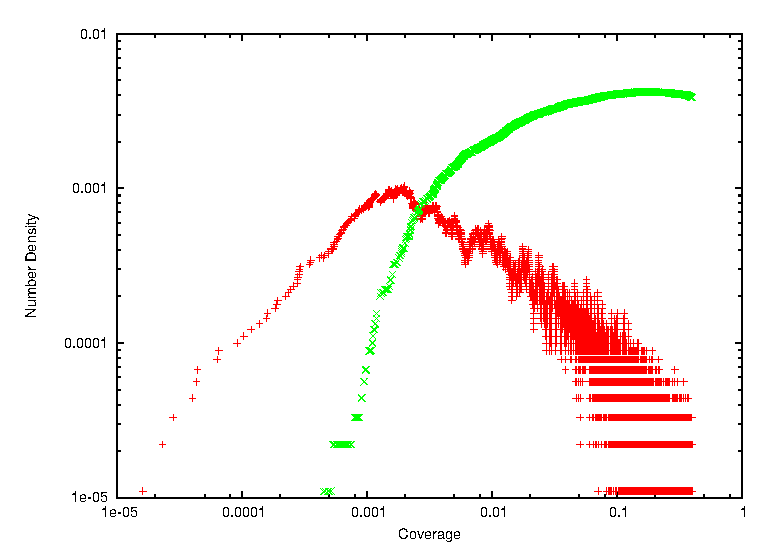
\includegraphics[width=\linewidth]{density.eps}
%\end{center}

\begin{center}
\begin{tabular}{cc}
\includegraphics[width=0.5\linewidth]{morph31.eps} &
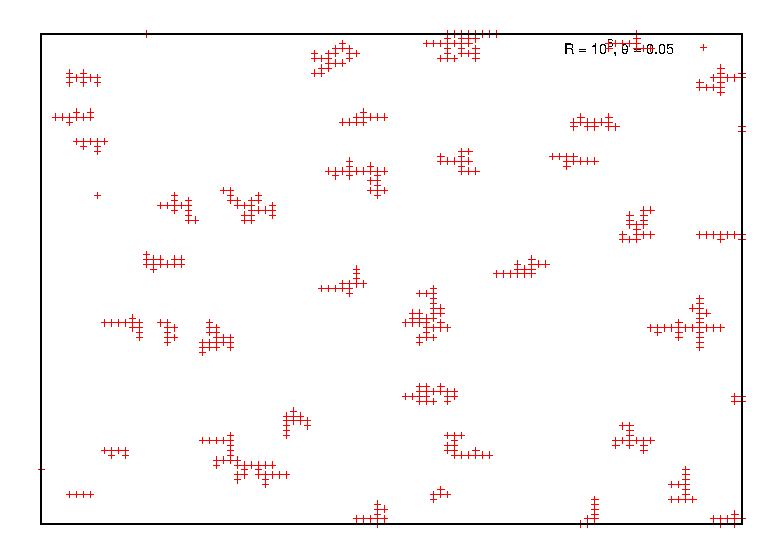
\includegraphics[width=0.5\linewidth]{morph32.eps} \\
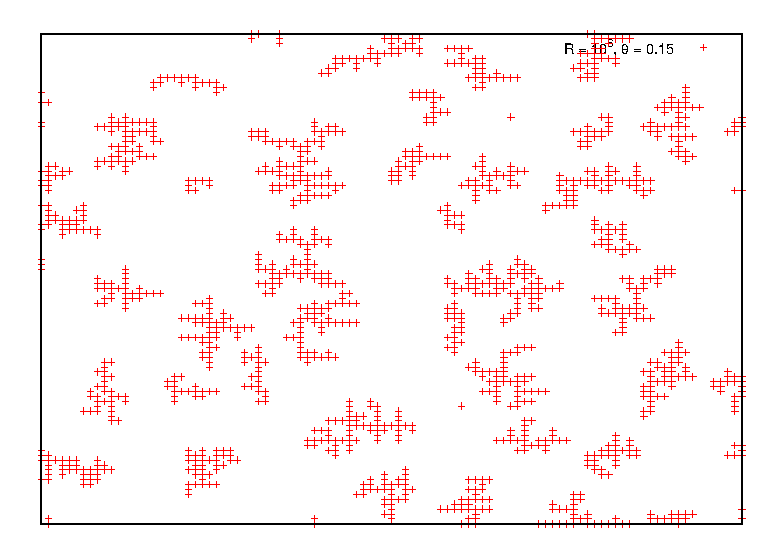
\includegraphics[width=0.5\linewidth]{morph16.eps} &
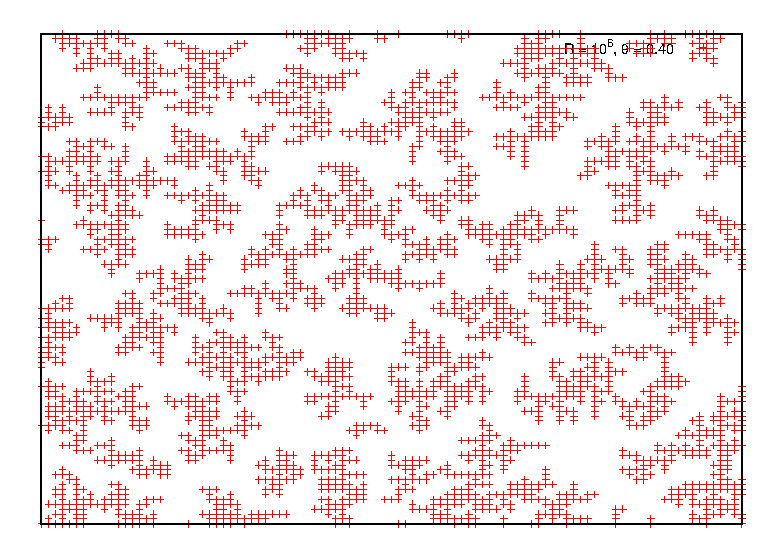
\includegraphics[width=0.5\linewidth]{morph24.eps} 
\end{tabular}
\end{center}
\end{textblock}

\begin{textblock}{20}(17,05)
\CHead{Scaling Theory}
It has been shown that the island distribution function can be written in the
form\cite{crit}
\[
	N_s(\theta) = \frac{\theta}{\langle s \rangle^2} 
	f_i\left(\frac{s}{\langle s \rangle}\right),
\]
where $N_s(\theta)$ is the number of islands of size $s$ per unit area for a
given coverage $\theta$, $\theta = Ft$ is the coverage, $s$ is island size, 
$\langle s \rangle$ is the
average size and $f_i$ is a universal scaling function for a given critical
island size $i$. By universal, we mean
that the function is independent of the coverage and of the growth parameters
$F$ and $D$. The scaling function should, however, be different for different
critical island sizes $i$. A functional form of the scaling funciton can be
obtained from the following assumptions\cite{crit}:
\begin{itemize}
\item the island size distribution behaves as $u^i$ for small $u$
\item the distribution has an exponential cuttoff for large $u$
\item the distribution peaks at the average island size ($u=1$)
\end{itemize}
These assumptions lead to the functional form
\[
	f_i(u) = C_i u^i e^{-ia_i u^{1/a_i}}.
\]
The constants $C_i$ and $a_i$ are determined by applying the sum rules
$\int f_i(u) ~du = \int u f_i(u) ~du = 1$,
which arise because the scaling function is really just a probability function
\cite{1d}.
The result of applying the sum rules to the above scaling functional form is
\[
	\frac{\Gamma[(i+2)a_i]}{\Gamma[(i+1)a_i]} = (ia_i)^{a_i}, 
	\quad C_i = \frac{(ia_i)^{(i+1)a_i}}{a_i \Gamma[(i+1)a_i]}.
\]

We propose a slightly different approach to the scaling function by
\textit{not} requiring the distribution to peak at the average island size, as
we see no constraint on this peak \textit{a priori}.
Keeping the rest of the assumptions leads to the much simpler scaling function
$f_i(u) = A u^i e^{-iub}$.
Again, the sum rules fix the values of $A$ and $b$, and the result is the
function
\[
	f_i(u) = \frac{(i+1)^{i+1} u^i e^{-(i+1)u}}{\Gamma(i+1)}.
\]
\end{textblock}

\begin{textblock}{15}(39,05)
\CHead{Results from Simulation}
\begin{center}
\centerline{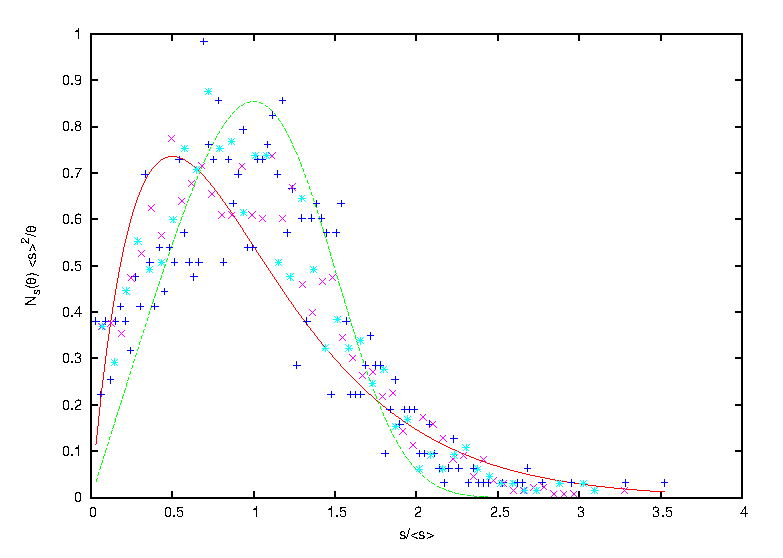
\includegraphics[width=\linewidth]{scale.eps}}
\end{center}

The above is a plot of the simulation data along with the two distribution
functions described previously. The simulation is a Monte Carlo technique based
on an algorithm proposed by Pablo Jensen \cite{pablo}. The plot contains
simulation data for values of $R=D/F$ ranging from $10^3$ to $10^6$ and for
coverages ranging from $0.05$ to $0.15$.

We see that the large
$s$ (large island size) regime is fit well by the newly proposed distribution
function; the small $s$ regime is less clear, and more simulation data based on
larger grid models is underway. Experimental results will be used
to charactize the distribution function as well.
\end{textblock}

\begin{textblock}{15}(39,19.5)
\CHead{Future Work}
More simulation data is needed to resolve the uncertainies seen above in the
small $s$ regime. Additionally, work needs to be done to verify the 
distributions for higher values of the critical island size $i$.

After verifying the scaling results in two dimensions, we would like to look at
the effects of deposition of not just monomers but of clusters as well (dimers,
trimers, etc.), corresponding to aggregation occuring in the vapor. 
Additionally,
diffusion through the liquid may become important as well.
\end{textblock}

\begin{textblock}{10}(22,22)
\small
\begin{thebibliography}{99}
\bibitem{crit}
	Jacques G. Amar and Fereydoon Family,
	Phys. \ Rev. \ Lett.\ {\bf 74}, \ 2066 (1995)

\bibitem{1d}
	J.A. Blackman and P.A. Mulheran,
	Phys. \ Rev. \ B. \ {\bf 54}, \ 11 681 (1996)

\bibitem{pablo}
	Pablo Jensen,
	Rev. \ Mod. \ Phys. \ {\bf 71}, \ 1695 (1999)
\end{thebibliography}
\end{textblock}

\begin{textblock}{54}(00,25.5)
\begin{center}
{\footnotesize Contact information:
Benjamin R. Hillman \ \ --
Phone: 425--218--8086\ \ --
Email: \url{benjaminr.hillman@gmail.com}
}
\end{center}
\end{textblock}

\end{document}
